\documentclass{article}

\usepackage[T1]{fontenc}
\usepackage[utf8]{inputenc}
\usepackage[frenchb]{babel}

\usepackage{hyperref}
\hypersetup{%
  colorlinks,%
  citecolor=black,%
  filecolor=black,%
  linkcolor=black,%
  urlcolor=black%
}

\usepackage{graphicx}

\usepackage{pgffor}
\usepackage{ifthen}
\usepackage{tikz}
\usetikzlibrary{matrix,fit,calc}

\usepackage{amsmath}
\usepackage[nottoc, notlof, notlot]{tocbibind}

\usepackage{rapport}

\author{Georges Dupéron}
\title{Langage de programmation}

\begin{document}

\maketitle
\tableofcontents
\newpage

\section{Objectif}

\subsection{Sujet}
Il y a environ 20 ans, le langage et le système d'exploitation FORTH avaient été mis au point, avec pour but de créer un environnement
totalement personnalisé pour chaque utilisateur. La particularité de FORTH était qu'il ne possédait pas de mots-clés, ou instructions
figées, et que chaque utilisateur était en mesure de définir lui-même ses propres primitives, voire redéfinir ses primitives... à
l'infini.

L'échec de FORTH est venu, entre autres de la nécessité d'échanger des programmes entre utilisateurs, et des conflits dus à l'homonymie
(même nom, fonction différente) et à la synonymie (même fonction, noms différents). %Également, l'évolution des besoins et
Les fonctions n'étaient pas toujours documentées, ce qui fait qu'un même programmeur ne pouvait pas faire exécuter, à un intervalle de
temps relativement court, 2 fois le même programme...

Pour autant, le côté adaptatif et souple de FORTH aurait été largement plébiscité s'il n'y avait eu cette difficulté. Une manière de
contourner ce genre de conflit, dû à une représentation symbolique textuelle trop fortement contrainte par la syntaxe, est de se pencher
vers une programmation qui privilégie les flux de données sur les actions à réaliser, et vers des bases graphiques plutôt que textuelles,
laissant donc à chaque utilisateur la liberté de définir ses actions, et préservant en revanche les flux.

L'idée de ce projet est de proposer une première architecture de compilateur ou d'interpréteur de premier niveau pour illustrer ce
paradigme, et tenter d'en évaluer les propriétés. Ce projet nécessite un excellent niveau en programmation et un goût prononcé pour
l'écriture de compilateurs.

\subsection{…}
%TODO IDE fait partie du langage
Le but de ce projet sera donc dans un premier temps de définir un langage de programmation visuel utilisant le paradigme du
dataflow\footnote{\url{http://en.wikipedia.org/wiki/Dataflow}}, et n'ayant pas de primitives fixes. Dans un second temps, nous
implémenterons un EDI\footnote{Éditeur de Développement Intégré} permettant de créer des programmes dans ce langage, et de les interpréter.

% TODO : fragment !!!
% Référecne perdue :(
Des recherches ont montré que dans le cadre des langages de programmation visuels, l'éditeur jouait un rôle aussi important que le langage
lui-même.

DSL = bien mais pas bien. Langages existants : ajout au vocabulaire (fonctions, variables), mais pas à la grammaire (structure) (sauf
macros, mais pas complètement). Nous on propose de permettre d'écrire de n'importe quelle manière (grammaire libre), tout en gardant la
possibilité d'ajout au vocabulaire. Nous ne gardons que les barrières nécessaires à une certaine cohérence (des éléments graphiques
connectés à d'autres). Les blocs peuvent être ronds, les traits annotés d'étiquettes, ou encore d'autres choses.

Graphes avec noeuds étiquetés et arcs éiquetés à chaque extrémité (et sur l'arc lui-même) => graphes généralisés.

Preuve de complétude de Turing : un graphe = des noeuds connectés par des arcs, un noeud = l'arc NULL ou qqch du genre. // $\lambda(\lambda(\dots))$.

L'interface utilisateur devient alors la même chose (fenêtres = blocs avec un affichage particulier).

\section{Formalisation du langage}

Dans cette section, nous allons essayer de trouver quelle est la nature, l'essence d'un programme, de manière à 

\subsection{Programme en dataflow}

Examinons un programme simple exprimé dans le paradigme du dataflow~:

\begin{figure}[h]
  \centering
  \begin{tikzpicture}
    \bloc[t]{+1/a+b}{ab}{c}
    \tikzset{+2/.style={below of=+1,matrix anchor=north}}
    \bloc[t]{+2/a+b}{ab}{c}
% \tikzset{b2/.style={right of=b1-out-d,matrix anchor=b2-in-x.center}}
%    \bloc[t]{b2/\frac{x\times y}{z}}{{x}{y}{z}}{{t}}
    
    \tikzset{e1/.style={left of=+1-in-a,matrix anchor=e1-out-val.center,input-bloc}}
    \bloc[t]{e1/e_1}{}{{val/}}
    \draw (e1-out-val) -- (+1-in-a);
    
    \tikzset{e3/.style={left of=+2-in-b,matrix anchor=e3-out-val.center,input-bloc}}
    \bloc[t]{e3/e_3}{}{{val/}}
    \draw (e3-out-val) -- (+2-in-b);
    
    \tikzset{e2/.style={at=($ .5*(e1-out-val) + .5*(e3-out-val) $),matrix anchor=e2-out-val.center,input-bloc}}
    \bloc[t]{e2/e_2}{}{{val/}}
    
    \node[coordinate] (between-+1-+2) at ($ .5*(+1-in-b) + .5*(+2-in-a) $) {};
    \node[coordinate] (connect-e2-+1-+2) at ($ .5*(between-+1-+2) + .5*(e2-out-val) $) {};
    
    \draw (e2-out-val) -- (connect-e2-+1-+2);
    \draw (connect-e2-+1-+2) |- (+1-in-b);
    \draw (connect-e2-+1-+2) |- (+2-in-a);
    
    
    \shorthandoff{:}
    \draw[->] (+1-out-c) -- ++(1,0) node[coordinate,label=above:\tiny$e_1+e_2$] {};
    \draw[->] (+2-out-c) -- ++(1,0) node[coordinate,label=below:\tiny$e_2+e_3$] {};
    \shorthandon{:}
  \end{tikzpicture}
  \caption{Un programme simple en dataflow.}
\label{fig:simple-dataflow}
\end{figure}

Ce programme a trois entrées ($e_1$, $e_2$, $e_3$), et deux sorties ($e_1+e_2$ et $e_2+e_3$).

\subsection{Caractéristiques du programme}
La question à se poser maintenant est ~:
\begin{figure}[h!]
  \centering
  Qu'est-ce qui définit ce programme ?
\end{figure}

Ou, comme le disait un des collègues de Joe~Armstrong~\cite{what-are-the-inputs}~:

\begin{figure}[h!]
  \centering
  \begin{quotation}
    «~A program is a black box. It has inputs and it has outputs. And there is a functional relationship between the inputs and the outputs. What are the inputs to your problem ? What are the outputs to your problem ? What is the functional relationship between the two ?~»
  \end{quotation}
\end{figure}

Ce programme est constitué
\begin{itemize}
\item d'entrées,
\item de sorties,
\item d'un graphe étiqueté exprimant la relation entre les sorties et les entrées grâce à des fonctions ($+$) qu'on suppose déjà définies,
\item d'une sémantique d'évaluation, qui donne une signification au graphe,
\item d'une représentation graphique,
\item Et pour l'exécuter pour de bon, il faut une machine réelle vers laquelle on peut compiler le programme (ou un interpréteur fonctionnant sur cette machine).
\end{itemize}

\subsection{Généralisation}
Si on généralise ce résultat, on peut dire qu'un programme est défini par une structure de données abstraite (on n'a pas besoin de connaître la représentation en mémoire de cette structure), qui peut contenir des entrées, des sorties, un arbre (ou graphe) syntaxique, etc. Cette structure peut être représentée sous forme d'un programme dont l'entrée est la désignation d'une partie de la structure que l'on souhite accéder, et dont la sortie est la partie en question.

La représentation graphique ou textuelle du programme peut être assurée par un autre programme.

Sa sémantique d'évaluation peut être définie par une machine abstraite, dont les (méta-)entrées sont le programme, ainsi que des entrées pour le programme, et dont les (méta-)sorties sont les sorties que le programme devrait avoir. Tiens ? Entrées, sorties, une relation fonctionnelle (les sorties sont celles du programme pour ses entrées), \dots\ Eh oui, notre machine abstraite, c'est-à-dire notre sémantique d'évaluation est bel et bien un programme elle aussi.

De même, la machine réelle vers laquelle on éspère pouvoir compiler le programme, peut être modélisée par un programme. Pendant que nous y sommes, rien ne justifie la présence de la machine réelle, car la machine abstraite pourrait très bien être la même que celle qui exécute le programme. C'est le cas par exemple si notre langage est le code machine d'un certain processeur : L'octet 0x12345678 a pour signification «diviser l'accumulateur par 2», c'est une définition de la sémantique du langage, et à la fois une définition de la machine qui exécute le programme.

La machine abstraite n'a donc pas besoin d'être si abstraite que ça, et pourrait être n'importe quelle machine, et il pourrait même y avoir plusieurs machines qui spécifient la sémantique du langage (de manière redondante, pour avoir le choix, et pour que ces définitions se vérifient mutuellement).

Et, pour continuer sur cette voie, il peut aussi y avoir plusieurs représentations syntaxiques (textuelle, avec ou sans coloration, graphique, \dots).

On a donc les équations suivantes dans le cas simple (une seule machine, une seule représentation) :

\begin{align}
  \text{Programme} &= \left\lbrace
      \begin{array}{rl}
          &\text{Type de données abstrait (ADT)}\\
        + &\text{Machine abstraite (sémantique)}\\
        + &\text{Représentation}
      \end{array}
      \right\rbrace\\
  \text{Programme} &= \text{Programme} + \mathrm{Programme} + \mathrm{Programme}\\
  \text{Programme} &= 3 \times \text{Programme}
\end{align}

\subsection{Base}

Nous voilà bien avancés\dots\ Un programme est un programme. C'est donc une définition récursive. Et toute définition récursive doit avoir une base, et des règles pour générer de nouveaux éléments. Nous venons de définir les règles, cherchons les bases possibles~:
\begin{itemize}
\item Machine de Turing
\item Lambda-calcul
\item Langage mathémathique
\end{itemize}

Le lambda-calcul et la machine de Turing sont
équivalents\footnote{\url{http://en.wikipedia.org/wiki/Lambda_calculus\#Computable_functions_and_lambda_calculus}}$\vphantom{X}^{,}$\footnote{Bien qu'ils ne
  semblent pas être totalement équivalents\cite{lambda-turing-equivalence}~: \quote{However, [Lambda Calculus] is not a model of computation for we
    cannot calculate an upper bound on resource consumption of its reduction steps without resorting to another model of computation, such
    as [Turing Machines] (according to Yuri Gurevich).}},
% http://conal.net/blog/posts/can-functional-programming-be-liberated-from-the-von-neumann-paradigm/#comment-35342
% A lambda calculus program does describe a computable function. However, LC is not a model of computation for we cannot calculate an upper
% bound on resource consumption of its reduction steps without resorting to another model of computation, such as TMs (according to Yuri
% Gurevich). But, models of computation don’t end there, either.
par contre le langage mathémathique permet d'exprimer des fonctions non-calculables, des ensembles infinis, et tout un tas de choses
obscures. Comme nos machines physiques actuelles sont une version bâtarde des machines de Turing (qui n'ont pas de limite sur la quantité de
mémoire disponible, contrairement aux notres), il semble sage de laisser de côté le langage mathémathique (pour l'instant, lorsque le
langage aura gagné en maturité, peut-être qu'il sera temps de l'ajouter).

L'équivalence $\lambda$-calcul vs. Turing nous laisse le choix pour l'implémentation de notre première machine à partir de laquelle les autres seront définies, directement ou indirectement. Explorons donc la suite du problème avant de prendre une décision. À terme, le meilleur sera probablement d'implémenter les deux, comme base, et de les définir mutuellement l'une à partir de l'autre, pour avoir une vérification.

\section{Notes pour la suite\dots}

% Suite
%Partir d'un plus haut niveau pour se faciliter la tâche : une VM simple en JahvaScript
%Définir une api de base (?), c'est une machine virtuelle sur laquelle s'exécuteront les programmes
%  - Structures de données
%  - Dataflow


%%%
%X Définir le langage grunt par rapport à une VM simple (et cette VM à partir d'une machine de Turing)
%  Prendre un programme grunt, et l'expanser au maximum (FORTH). Descendre jusqu'au niveau des transistors ou au moins des bascules.

Nous allons prendre un programme en dataflow, et le déconstruire le plus possible, afin de voir quelles sont les «primitives» sémantiques nécessaires à notre langage. Bien que FORTH n'ait pas à proprement parler de primitives, il a lui aussi une sémantique (chaque mot est expansé en la suite de mots le définissant, jusqu'à arriver au code machine).
  

Il faut définir un bloc eager-evaluation, qui prend en paramètre un graphe, et
\begin{itemize}
\item Soit le réécrit (compilation)
\item Soit l'évalue (interprétation)
\end{itemize}
Dans le cas où on compile, on aura une "instruction" call-bloc

call-bloc prend en paramètre des fonctions permettant de calculer ses paramètres, ainsi que les paramètres eux-mêmes.
\begin{itemize}
\item En évaluation paresseuse, on n'évalue les paramètres que s'ils sont nécessaires.
\item En évaluation «eager», on évalue les paramètres au début de l'appel du bloc, et on stocke leur valeur pour une future utilisation (ou non).
\item Pour une macro, on stocke juste les paramètres eux-mêmes (avec leur fonction d'évaluation, s'il y en a une).
\end{itemize}

\section{Implémentation}
Pour l'implémentation, nous nous limiterons à un sous-ensemble purement fonctionnel du langage défini dans les sections suivantes.

\appendix

\section{notes}
\begin{itemize}
\item code bubbles
\item dataflow
\item world machine
\item vidéo alan kay
\item pas de conflits de nommage
\item gruntnetwork.com
\item Design patterns
\item Domain Specific Language
%% \item relire le sujet !!!
\item DSL
\item vue «libre»
\item thèse sur la programmation par l'exemple
\item Preuves
\item Spécification fonctionnelle
\end{itemize}

\begin{figure}[H]
  \centering
  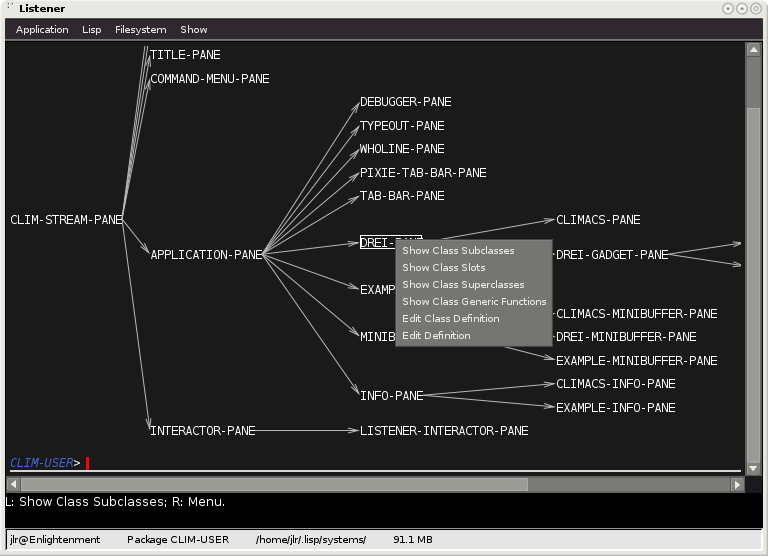
\includegraphics[width=10cm]{lisp-class-graph}
  \caption{Graphe d'héritage des classes en Lisp avec McCLIM}
  % On http://mcclim.cliki.net/Screenshot : http://jlr.freeshell.org/data/mcclim/screenshots/2007-03-27-listener-dark-classgraph-context-menu.png
  % http://boinkor.net/lisp/porn/clim-debugger.png
\label{fig:lisp-class-graph}
\end{figure}
\subsection{Historique}
\begin{itemize}
\item Control flow graphs
\item alsa «composer»
\item http://recherche.ircam.fr/equipes/repmus/RMPapers/CMJ98/
\item Pourquoi dataflow peu utilisé ? (chest hair ?, http://therighttool.hammerprinciple.com/, contacter l'auteur pour qu'il ajoute des VPL)
\end{itemize}

\nocite{*}
\bibliographystyle{plain}
\bibliography{biblio}

\end{document}
